\documentclass[../diplomski_rad.tex]{subfiles}

\begin{document}

\sloppy

\justifying

%uvod u poglavlje
Analiza bioelekričke impedancije je neinvazivna metoda kojom se procjenjuje sastav ljudskog tijela. 
Kroz tijelo se pušta slaba struja te se mjeri pad napona čime se izračunava impedancija tijela. 
Mjerenjem bioimpedancije moguće je praćenje kretanja tekućina kroz tijelo što je vrijedna dijagnostička metoda za praćenje stanja srčanih bolesnika. 

\section{Sastav ljudskog tijela}

Ljudsko tijelo je kompleksna biološka struktura koja se sastoji od različitih međusobno povezanih tkiva koja 
omogućavaju funkcioniranje organizma. Tkiva se približno sastoje od 
64\% vode,
20\% proteina,
10\% masti 
i 5\% minerala. 
Valja napomenuti kako na sastav ljudskog tijela utječu pojedini faktori, kao što su spol i dob \cite{Bera2014}.  

Procjena sastava ljudskog tijela pruža važne informacije koje se koriste u praćenju zdravlja, 
procjeni rizika od pojedinih bolesti, praćenju oporavka te ranom otkrivanju zdravstvenih problema. 

Voda je osnovni element stanica i tkiva te je nužna za brojne fiziološke procese u organizmu, 
kao na primjer održavanje elektrolitske ravnoteže i regulacija temperature.
Ukupnu vodu u tijelu (engl. \textit{Total Body Water; TBW}) 
dijelimo na intracelularnu vodu (engl. \textit{Intracellular Water; ICW}) i ekstracelularnu vodu (engl. \textit{Extracellular Water; ECW}). 
Važni parametri pri analizi ljudskog tijela su i masa tijela bez masnog tkiva (engl. \textit{Fat Free Mass; FFM}) 
te masa masnog tkiva (engl. \textit{Fat Mass; FM}) \cite{Bera2014}.

Ekstracelularna voda je količina vode koja se nalazi izvan stanica te čini 30-40\% ukupne vode. Uključuje krv, limfu, tekućinu u 
zglobovima i međustaničnom prostru. Ima važnu ulogu u transportu kisika i hranjivih tvari do stanica te odvođenju otpadnih 
tvari iz organizma \cite{Bera2014}.

Intracelularna voda je voda koja se nalazi unutar stanica. Ona čini 60-70\% ukupne vode u tijelu. 
Ključna je za mnoge biološke procese unutar stanica, kao na primjer održavanje ravnoteže elektrolita. 
Održavanje ravnoteže između ekstracelularne i intracelularne vode ključno je za normalno funkcioniranje organizma \cite{Bera2014}.

Masno tkivo je također važno za funkcioniranje organizma jer pruža energetsku rezervu, toplinsku izolaciju te štiti unutarnje organe. 
Prekomjerno nakupljanje masnoće može dovesti do različitih zdravstvenih problema, poput pretilosti, dijabetesa i 
bolesti kardiovaskularnog sustava. 
Zbog toga je praćenje udjela masnog tkiva u organizmu važno u procijeni rizika od brojnih bolesti \cite{Bera2014}.

Masu tijela bez masnog tkiva dobijemo tako da od ukupne mase tijela oduzmemo masu masnog tkiva. 
FFW uključuje tjelesnu vodu, mišiće, kosti, organe i druga tkiva osim masnih tkiva te predstavlja masu koja je aktivna i sudjeluje 
u metaboličkim procesima \cite{Bera2014}.

Koliko dobro će tkivo provoditi struju, ovisi o količini vode u njemu. 
Tkiva koja imaju više vode u sebi, kao na primjer mišići, bolje provode eletričnu struju nego masno tkivo koje ne sadrži vodu. 
Zbog toga se sastav ljudskog tijela procjenjuje iz izmjerene bioimpedancije između različitih dijelova tijela. 
Iz bioimpedancije sastav tijela se dobiva putem teorijskih jednadžbi ili tablica koje ovise o parametrima 
kao što su spol, dobna skupina, težina i visina.

\section{Modeliranje bioimpedancije}

Bioimpedancija predstavlja električni otpor koji se javlja kada kroz biološka tkiva teče električna struja.
Ovisna je o frekvenciji te se može prikazati formulom:
\begin{equation}
    \label{jed:cpe}
    Z(f) = R_{e}(f) + jI_{m}(f) = |Z(f)|\angle\theta(f) 
\end{equation}
gdje je
\begin{equation}
    \label{jed:cpe}
    |Z(f)| = \sqrt{R_{e}^{2} + I_{m}^{2}}
\end{equation} 
\begin{equation}
    \label{jed:cpe}
    \theta(f) = arctg(\frac{I_{m}}{R_{e}})
\end{equation} 

U slijedećim potpoglavljima dan je pregled korištenog modela za modeliranje bioimpedancije ljudskog tijela.

\subsection{Električki model ljudkog tijela}

Ljudsku stanicu možemo modelirati ekvivalentnom električkom RC mrežom \cite{Lukaski2013} kako je prikazano na slici (referenca na sliku).

-slika ona stanice ide tu

Stanična membrana zbog svojih kapacitivnih svojstava propušta struju visokih frekvencija, dok struje niskih frekvencija blokira. 
Zbog toga postoji razlika u mjerenoj impedanciji u ovisnosti o frekvenciji uzbudne struje.  


\subsection{Matematički model bioimpedancije}

Matematički model kojim se najčešće modelira bioimpedancija ljudskog tijela naziva se Cole model. 
Razvio ga je britanski fizičar Kenneth Cole 1940-tih godina. 
Cole model opisuje impedanciju tijela kao funkciju frekvencije zbog cega ga koristimo pri analizi sastava ljudskog tijela \cite{Freeborn2021}.

\begin{figure}[htb]
    \centering
    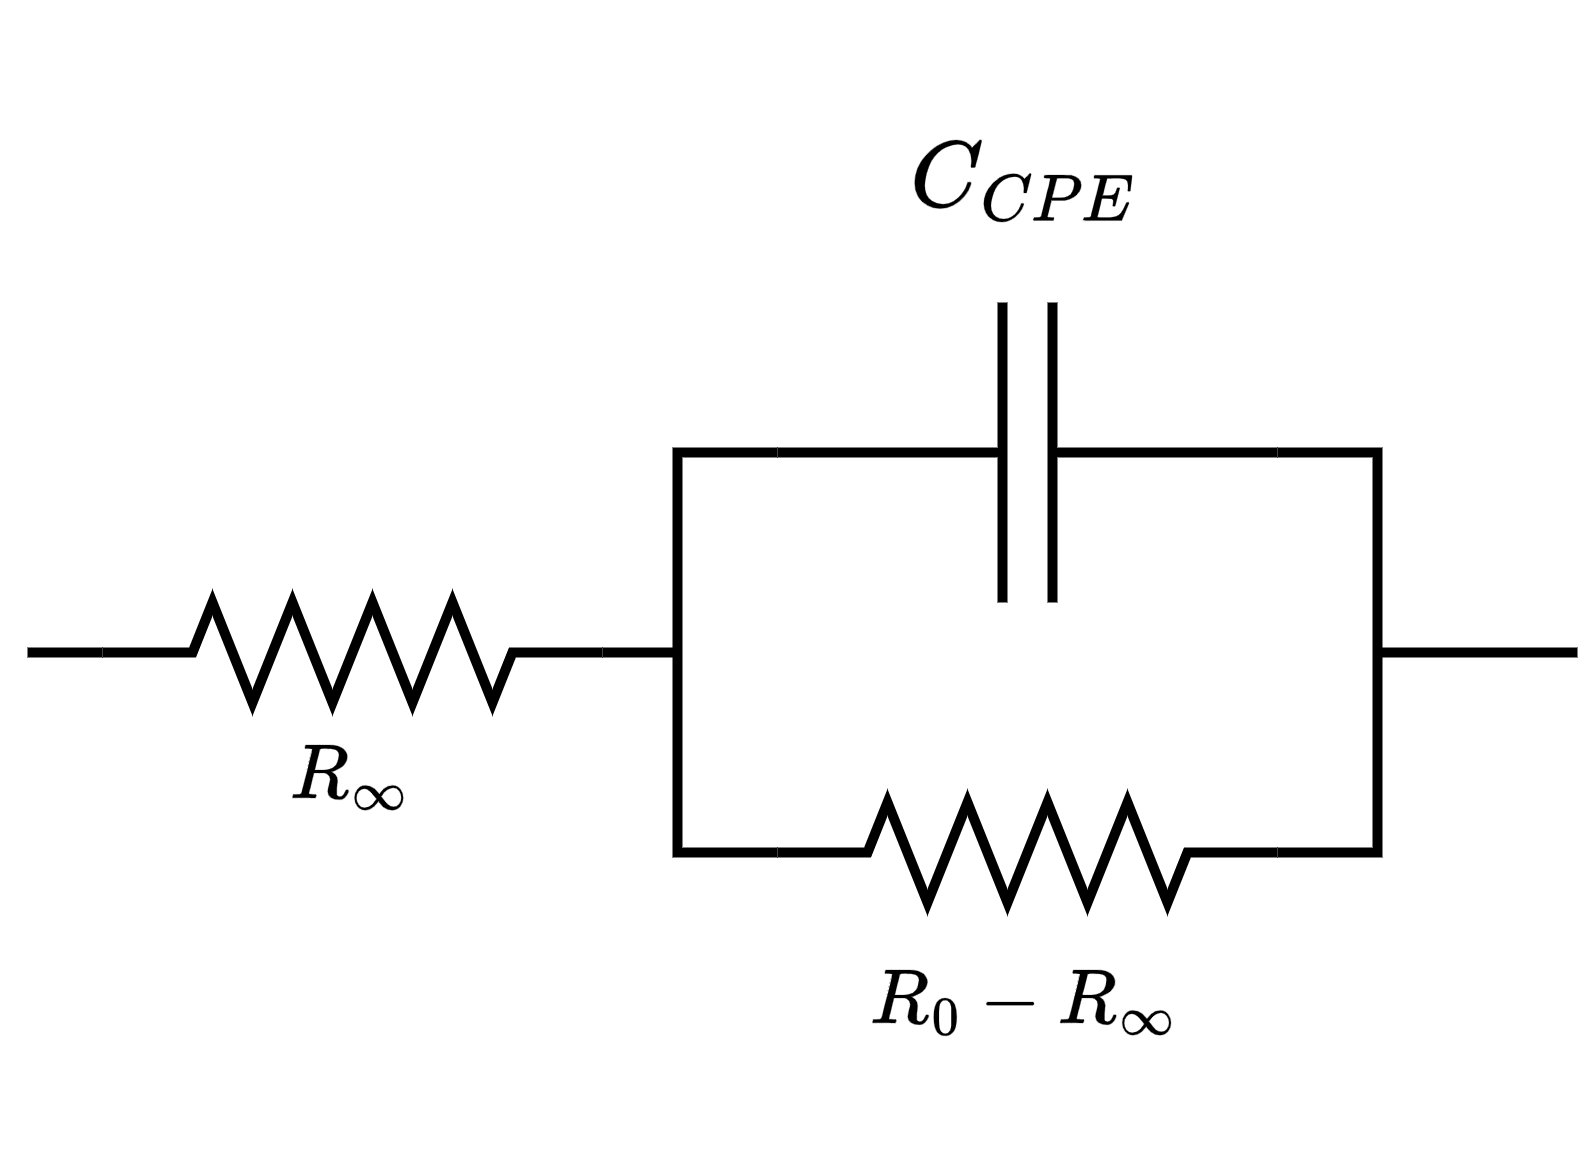
\includegraphics[width=0.6\textwidth]{Figures/cole_model.png} 
    \caption{Cole model bioimpedancije}
    \label{slk:cole_model}
\end{figure}

$R_{\infty}$ prestavlja otpor tkiva na beskonačnoj frekvenciji dok $R_{0}$ prestavlja otpor na nultoj frekvenciji. 
Razlika otpora $R_{\infty}-R_{0}$ prestavlja dodatan otpor struji na niskim frekvencijama zbog nepropusnosti stanične membrane. 
$C_{CPE}$ je element s konstantnom fazom koji modelira kapacitivnost stanične membrane 
te predstavlja neidealan kondenzator. Njegova impedancija iznosi: 
\begin{equation}
    \label{jed:cpe}
    Z_{CPE}(\omega) = \frac{1}{(j\omega)^{\alpha}C}
\end{equation} 
gdje je C kapacitet, a $\alpha$ njegov red. Kada je $\alpha = 0$ element s konstantnom fazom predstavlja idealan otpornik, 
dok sa $\alpha = 1$ predstavlja idealan kondenzator. 
Tipične vrijednosti parametra $\alpha$ za biološka tkiva su u intervalu 0.5 $< \alpha <$ 1 \cite{Freeborn2021}.

Ako uvedemo karakterističnu vremensku konstantu $\tau$ kao
\begin{equation}
    \label{jed:time_const}
    \tau = [(R_{0}-R_{\infty})C]^{1/\alpha}
\end{equation}
dobivamo orginalnu jednadžbu Cole modela: 
\begin{equation}
    \label{jed:cole}
    Z(\omega) = R_{\infty}+\frac{R_{0}-R_{\infty}}{1+(j\omega\tau)^{\alpha}} 
\end{equation} 
Iz jednadžbe \ref{jed:cole} vidljivo je kako su parametri Cole modela bioimpedancije 
$R_{\infty}$, $R_{0}$, $\alpha$ i $\tau$. 
Svojstva tkiva opisuju se pomoću ta četiri parametra, a postupak kojim se do njih dolazi opisan je u daljnjem tekstu.

\subsection{Graf bioimpedancije Cole modela}
Ovo tu je glupo, dvaput spominjes isto!!!
Rezultati mjerenja bioimpedancije na razilčitim frekvencijama mogu se aproksimirati polukružnicom,  
što je prikazano na slici \ref{slk:cole_graf}. 
Graf bioimpedancije Cole modela je polukružnica koja prikazuje omjer negativne reaktancije i otpora tkiva na svim frekvencijama, 
od $f=0$ do $f=\infty$. Frekvencija raste s desna na lijevo. 

\begin{figure}[htb]
    \centering
    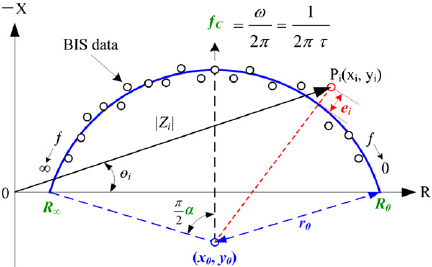
\includegraphics[width=0.7\textwidth]{Figures/cole_plot.png} 
    \caption{Graf bioimpedancije Cole modela \cite{Yang_2013}}
    \label{slk:cole_graf}
\end{figure}

Iz opisanog grafa moguće je dobiti parametre Cole modela\cite{Yang_2013}.
$R_{\infty}$ i $R_{0}$ jednostavno se isčitavaju kao precjesišta polukružnice i realne osi.
Vremenska konstanta $\tau$ inverz je karakteristične kružne frekvencije $\omega_{C}$ na kojoj je reaktancija najveća.
Relacija iz koje se izračunava $\tau$ je:
\begin{equation}
    \label{jed:cole}
    f_{C} = \frac{\omega_{C}}{2\pi} = \frac{1}{2\pi\tau} 
\end{equation} 
Parametar $\alpha$ određuje koliko je središte kružnice pomaknuto ispod realne osi. 
Izračunava se iz kuta između karakteristične frekvencije $f_{C}$ i beskonačne frekvencije $f_{\infty}$. 
Ako se taj kut definira kao $\theta$, vrijedi sljedeći izraz:
\begin{equation}
    \label{jed:cole}
    \theta = \frac{\pi}{2}\alpha 
\end{equation} 

\end{document}